% !Mode:: "TeX:UTF-8"


\externaldocument{chap3}

\chapter{基于时空互表征学习的鲁棒多目标跟踪方法}
\label{chap:stml}


\section{引言}
随着智能化时代的进入,视频多目标跟踪任务得到了巨大的重视并应用到了社会的各个方向。
% STURE: Introduction
在线多目标跟踪已成为智能驾驶~\cite{geiger2012are} 、动作识别~\cite{RN583} 等实时应用所必需的关键科学问题和感知技术。
虽然近些年多目标跟踪算法取得了一些的进展,但因为场景的动态开放和相互干扰等问题的普遍性,使动态开放场景下的多目标跟踪问题依然具有挑战,
所以提出一个高效的多目标跟踪算法来提升模型的速度和精度具有十分重大的价值。

考虑到现实场景的动态开放性,多目标跟踪任务本质上是复杂的,多目标跟踪中的关键难点是同一目标的外观变化、不同目标的相似外观和一组目标的频繁遮挡等。
随着深度学习的发展,多目标跟踪取得了巨大的进步~\cite{RN550,wen2020ua-detrac}。
多目标跟踪算法通过定位和识别连续帧中的多个目标来生成一致的轨迹,一般可以分为两类:离线和在线多目标跟踪方法。
离线多目标跟踪方法可以利用整个视频信息来提取跟踪结果,
但并不适合智能驾驶等在线应用,
而在线多目标跟踪方法仅使用到达当前时刻可获取的数据。

\begin{figure*}[ht]
	\centering
	\includegraphics[width=0.87\textwidth]{./figures/C4Fig/introduction.pdf}
	\vspace{0.2em}
	\caption{时空互表征学习和鲁棒的目标关联}
	\label{fig:sture_introduction}
\end{figure*}

由于目标检测精度~\cite{ren2017faster}的提高,将当前检测结果与历史序列相关联的数据关联方法得到了广泛应用。
但是数据关联算法过于依赖于完美的检测结果,一旦跟踪目标的检测结果丢失、忽略或不准确,跟踪过程很可能会失败。
这些问题可以通过遵循跟踪预测范式,使用最新的高精度单目标跟踪器~\cite{RN1215,RN1212,RN1214} 来缓解。
单目标跟踪器仅使用第一帧目标的检测结果来预测后面序列帧中被跟踪目标的位置和大小~\cite{li2016robust}。
然而,当被跟踪物体被其它干扰物遮挡时,这些单目标跟踪器会产生漂移~\cite{RN717,2021Person}。
为了弥补跟踪预测范式的缺点,本章采用了一种将数据关联方法的优点与单目标跟踪器相结合的方法,使用一系列单目标跟踪器来跟踪大多数视频帧中的目标,
当跟踪的分数低于阈值时,将使用目标关联方法解决漂移问题,以提高多目标跟踪的性能。


此外,多目标跟踪中的数据关联是指将当前帧候选检测结果与一系列历史轨迹进行匹配关联~\cite{RN994,RN724},
并且历史轨迹通常包含一个具有时间特征的目标序列,而候选检测结果只包含一个平坦的目标图像特征,而数据关联又必须在两种不同形态(分别是单个检测结果和图像序列)之间进行目标关联。
%多项研究~\cite{RN969,RN970} 表明,
从第~\ref{chap:nonlocal} 章的研究以及一些其他工作~\cite{RN969,RN970} 可以看出,从图像序列中提取时间特征可以在各种动态开放环境中获得更鲁棒的目标序列特征。
然而,这些方法忽略了当前检测图像在数据关联期间缺乏时间特征,因此当前帧的检测结果不能利用时间特征。
如图~\ref{fig:sture_introduction} 所示,当前检测的空间特征缺乏针对历史序列的时间特征,它只关注了显著目标的部分区域。
当前候选检测结果和历史轨迹之间的特征不平衡问题使得计算数据关联中的相似性变得更加困难。
因此,设计一种利用历史的时间信息来增强当前检测特征的方法显得尤为紧迫和重要。

为了解决当前检测结果的时间特征被忽略的问题,即数据关联双方特征不平衡的问题,本章引入了一种新颖的时空互表征学习(Spatial-Temporal  mUtual REpresentation learning,STURE)方法。
受到互学习策略~\cite{RN983} 的启发,该策略在整个训练过程中双方协作地进行特征学习。
空间信息由检测学习网络进行提取,通过所提出的 STURE 方法,序列学习网络学习的时间信息被转移到检测学习网络。
在训练阶段,给定一个目标序列,强制检测学习网络学习到的当前检测特征去逼近和拟合序列学习网络学习到的历史轨迹特征。
通过使用 STURE,序列学习网络和检测学习网络相互学习这些时空特征。
在测试阶段,使用强化后的检测学习网络提取当前检测的特征。
受益于所提出的时空互表征学习方法,抽取历史序列的时间特征以增强当前检测结果的空间特征,增强的检测特征可以更加全面的关注显著目标。
由于学习到了时间信息,使得当前检测特征对各种动态开放环境具有较好的鲁棒性,就像图~\ref{fig:sture_introduction} 中的强化后的特征一样。
该方法解决了检测与序列特征差异的问题,使得当前候选检测结果在数据关联上可以更好地与历史轨迹进行关联。

综上所述,本章的主要贡献如下:
\begin{itemize}
	\item  提出了一种新颖的 STURE 架构来解决数据关联中当前检测结果的空间特征与历史序列的时空特征之间的特征不平衡问题。
	\item  为了增强所提出方法的互学习和识别能力,设计了三个合理的损失函数:交叉损失、形态损失和相似性损失,这将有助于检测学习网络获得历史轨迹的时间特征。
	\item  设计了一种基于预测的多目标在线跟踪范式,通过使用经过 STURE 增强的特征来缓解单目标跟踪器的漂移问题,这将提高所提出方法的准确性和鲁棒性。
	\item  在多目标跟踪基准数据集上进行的大量实验和消去研究表明,与最先进的在线多目标跟踪方法相比,所提出的算法可以获得较好的跟踪性能。
\end{itemize}


\section{相关工作}
本章主要提出了一种基于时空互表征学习的鲁棒目标关联多目标跟踪方法,
因此本节将简单地讨论与之相关的多目标跟踪、时空建模和互学方法。

\subsection{多目标跟踪}
目前多目标跟踪方法通常涉及目标关联,一般遵循基于检测关联的跟踪范式。
例如,通过计算当前帧检测结果和历史帧轨迹的亲和度来进行跨帧关联。
根据是否采用整个视频信息,多目标跟踪方法分为在线和离线跟踪方法。
离线方法~\cite{tang2017multiple,RN973} 利用历史和未来信息,因此它们可以利用有关整个视频序列的信息。
他们通常将多目标跟踪建模为具有不同范式的图优化问题~\cite{li2020graph},例如 $k$ 部图~\cite{dehghan2015gmmcp} 或者多割~\cite{tang2017multiple}。

而在线多目标跟踪方法~\cite{chu2017online, RN974, RN1004, junbo2020a} 不利用未来的信息,但是当跟踪目标的检测结果不准确时很可能会失败。
以前的大多数方法~\cite{bae2014robust,xu2019spatial-temporal}采用逐检测并跟踪的流程,其性能在很大程度上取决于检测结果好坏。
其它一些方法~\cite{RN1004,RN455,RN542} 则是利用单目标跟踪器来进行在线多目标跟踪,通常会获得更好的效果。

在这项研究中,引入了一种相似性关联方法和基于预测跟踪的范式来处理检测结果不完美的问题。
这表明与现有算法相比,新的多目标跟踪方法可以获得更好的跟踪结果。


\subsection{时空建模}
提取时空特征对于序列帧特征建模非常重要。
通常,用循环结构进行时间特征的提取~\cite{chung2017a, mclaughlin2016recurrent, RN977}。
在每个时间步使用时间平均池化~\cite{mclaughlin2016recurrent} 来提取视频序列的特征。
然而,这些方法不能处理多个相邻区域。
最近,非局部神经网络被用来模拟长期的时间关系~\cite{RN580}。
 
对于在线多目标跟踪,稳健的运动表征对于目标关联很重要。
最近已经形成了很多使用深度神经网络的在线多目标跟踪方法~\cite{chu2017online,RN455,RN601}。
例如,孪生网络~\cite{leal-taixe2016learning} 通过聚合目标外观和光流信息来估计当前检测结果和历史轨迹的亲和力。
特别是可以利用长短时记忆网络提取空间表征~\cite{RN455},它一一处理序列中的检测结果并输出它们之间的相似性。
在这项研究中,使用自注意机制来提取目标序列中的时间特征。


\subsection{互学习}
一般来说,互学习~\cite{RN979,hinton2015distilling,romero2015fitnets,RN982} 是贯穿整个模型训练过程的一种广泛使用的合作式学习方法。
对于互学习方法,该过程通常是通过优化来自两个不同网络输出分布之间的~KL~散度来进行的~\cite{hinton2015distilling,RN983}。
此外,还可以优化两个网络的中间层输出~\cite{romero2015fitnets}。
特征迁移是通过计算度量学习问题~\cite{RN982, RN984} 中跨样本的相似度来进行的。
在研究中,通过优化当前检测特征与历史序列特征在互表征空间中的损失来相互学习时间特征。
损失函数的设计参考行人再识别方法~\cite{RN927},将其用于新的模型架构。
此外,交叉损失是根据互表征空间的差异而设计的。
序列学习网络和检测学习网络是同步训练的,而不是单独进行训练。
在多目标跟踪方法中,本章所提出的 STURE 方法是多目标跟踪领域首次尝试在互表征空间中训练序列学习网络和检测学习网络。


\vspace{0.5em}
\begin{figure*}[ht]
	\centering
	\includegraphics[width=1.0\textwidth]{./figures/C4Fig/network.pdf}
	\vspace{0.2em}
	\caption{多目标跟踪数据关联中 STURE 方法的体系结构}
	\label{fig:sture_network_architecture}
\end{figure*}

 

\section{时空互表征学习架构}
本章将详细介绍用于多目标跟踪数据关联中的时空互表征学习体系架构。
首先,展示了 STURE 的完整模型架构概述。
其次,给出了检测学习网络和序列学习网络的详细信息。
然后,介绍了训练损失函数的设计和模型训练方法。
最后,说明如何利用训练好的模型将当前检测和在线多目标跟踪中的历史轨迹关联起来。

\subsection{架构概述}
如图~\ref{fig:sture_network_architecture} 所示是检测结果和目标序列数据关联中 STURE 的详细架构。
不同的颜色表示不同的信息传递路径。
蓝色路径表示通过序列和检测之间的特征差异计算交叉损失 $L_C$,而灰色路径表示通过检测序列和单个检测之间的形态差异计算形态损失 $L_M$。
此外,相似性损失 $L_S$ 用于训练序列学习网络 $\mathcal{F}_{seq}(\cdot)$ 和检测学习网络 $\mathcal{F}_{det}(\cdot)$。
具体来说,时空特征是同时学习的。
最后,根据历史目标序列与当前检测的相似度进行在线数据关联。
序列学习网络学习空间特征并同步处理序列帧之间的时间关系,同时检测学习网络学习当前检测的空间特征。
通过序列学习网络和检测学习网络在时空互表征空间中利用设计的损失函数提取时空特征。
通过优化总目标函数,检测表征和序列表征将同时被学习到。
最后根据历史轨迹与当前检测结果的相似度进行检测结果到序列轨迹目标的关联。
详细过程在以下部分中介绍。


\subsection{时空建模网络}

\subsubsection{序列学习网络}

为了在单个模型中提取历史目标轨迹的时空特征,本章的序列学习网络借鉴了第~\ref{chap:nonlocal} 章中具有非局部自注意机制的卷积神经网络。
通过利用序列内的时间关系,非局部注意力神经网络可以将图像特征汇总为单个特征,然后使用输入特征~\cite{RN580} 对每个位置的激活进行加权平均值。
\vspace{0.5em}
\begin{figure*}[ht]
	\centering
	\includegraphics[width=0.6\textwidth]{./figures/C4Fig/sequence.pdf}
	\vspace{0.2em}
	\caption{序列学习网络的架构}
	\label{fig:sture_sequence}
\end{figure*}
 
图~\ref{fig:sture_sequence} 中表示的是基于 ResNet 的序列学习模型的架构。
所有输入的 8 张检测图像构成输入序列,每个目标的尺寸大小为 $256\times 128$,序列学习网络的输出为 $1\times2048$。
五个非局部注意力块嵌入到卷积神经网络中,
并删除最后卷积中 ResNet 的最后下采样操作,以获得高分辨率的特征图~\cite{RN985}。
对于 $N$ 个目标序列 $\mathcal{S}=\{S_n\}^N_{n=1}$,可以形式化描述为:
\begin{equation}\label{eq:pedestrian_sequence}
S_n=\{F_{n1},F_{n2},...,F_{nT}\}\mbox{,}
\end{equation}
其中 $n$ 是目标序列的索引,$n=1,2,...,N$,这里的 $T$ 是每个目标序列的帧数。
所以序列特征可以通过模型 $\mathcal{F}_{seq}(\cdot)$ 得到:
\begin{equation}\label{eq:sequence_network}
\left( f_{n1},f_{n2},...,f_{nT} \right)=\mathcal{F}_{seq}(S_n)\mbox{,}
\end{equation}
其中 $f_{nt} \in R^{D}$ 是 序列 $S_{n}$ 中帧 $F_{nt}$ 的特征,$t=1,...,T$。
许多目标序列特征通过使用三维平均池化被压缩为单个序列表征 $f_{Sn}\in R^{D}$:
\begin{equation}\label{eq:tap}
f_{Sn}=TAP\left( f_{n1},f_{n2},...,f_{nT} \right)\mbox{。}
\end{equation}
		
\subsection{检测学习网络}
为了学习空间特征,检测学习网络使用移除了最后一个全连接层的残差网络~\cite{he2016deep}。
同时,为了获得更高的空间分辨率和更精细的检测特征,像序列学习网络一样删除了 ResNet-50 的最后一个下采样操作。
如果忽视目标序列之间的时间特征,输入序列 $\mathcal{S}$ 可以看作是许多独立的检测 $\{F_{nt}\}_{n=1,t=1}^{N, T}$。
因此检测学习网络 $\mathcal{F}_{det}(\cdot)$ 用于学习独立检测结果的特征,第 $t$ 个序列中的第 $n$ 个检测特征可以表示为:
\begin{equation}\label{eq:detection_network}
d_{nt}=\mathcal{F}_{det}(F_{nt}),
\end{equation}
其中 $d_{nt}\in R^{D}(t=1,...,T)$ 为序列帧 $F_{nt}$ 对应的检测特征,$t=1,2,..,T$。

序列学习网络和检测学习网络的主干网络都是深度残差网络,
它们之间唯一的区别是前者增加了额外的非局部神经网络来提取时间特征。


\subsection{时空互表征学习}
一般对于在线多目标跟踪,数据关联的结果与学习到特征的鲁棒性有很大关系。
在目标序列中提取时间知识会提高空间特征在各种环境挑战中的鲁棒性~\cite{RN986}。
然而,输入为平面图像的检测学习网络没有包含时间特征,故无法有效处理时间相关性,这降低了它应对动态开放环境的能力。
为了解决这个问题,所提出的 STURE 方法使检测学习网络的输出与序列学习网络的输出在互表征空间中相匹配。

对于特定的目标序列 $S_n$,利用方程~\ref{eq:sequence_network}、方程~\ref{eq:tap} 和 方程~\ref{eq:detection_network} 提取序列特征 $f_{ Sn}$ 和检测特征 $d_{nt}$。
因为 $\mathcal{F}_{seq}(\cdot)$ 学习目标序列 $F_{nt}$ 之间的空间特征和时间相关性,所以 $f_{Sn}$ 包含空间特征和时间特征。
为了在检测学习网络和序列学习网络中相互提取序列的时间特征表示 $f_{Sn}$,STURE 旨在优化以下损失。


\subsubsection{交叉损失}
STURE 强制检测学习网络在互表征空间中匹配更精细更鲁棒的时间特征。
在这种情况下,使用 STURE 以缩小目标序列表征和相应检测表征之间的形态差异。
它在序列学习网络和检测学习网络中利用深度特征相互学习时间特征。
目标特征的表征用交叉样本表示。
整个目标序列的特征可以描述为 $\{f_{nt}\}_{n=1,t=1}^{N,T}$ 。
使用交叉样本来衡量检测-检测、检测-序列、序列-序列之间的特征差异,
交叉样本的欧氏距离矩阵 $M^{seq}\in R^{NT\times NT}$ 可以表示为:
\begin{equation}\label{eq:m_seq}
M^{seq}={
	\left[ \begin{array}{cccc}
	m_{11} & m_{12} & ... & m_{1N}\\
	m_{21} & m_{22} & ... & m_{2N}\\
	... & ... & ... & ... \\
	m_{N1} & m_{N2} & ... & m_{NN}\\
	\end{array} 
	\right ]}\mbox{,}
\end{equation}
其中每个子矩阵 $m_{ij} (i,j=1,2,...,N)$ 都是大小为 $T \times T$ 且具有相同值的矩阵。
其中,$T$ 是目标序列的长度,$N$ 是序列的数目。
\begin{equation}\label{eq:m_ij}
m_{ij}={
	\left[ \begin{array}{cccc}
	s_{ij} & s_{ij} & ... & s_{ij}\\
	s_{ij} & s_{ij} & ... & s_{ij}\\
	... & ... & ... & ... \\
	s_{ij} & s_{ij} & ... & s_{ij}\\
	\end{array} 
	\right ]},
\end{equation}
其中 $s_{ij}$ 是序列 $i$ 和序列 $j$ ($i,j=1,2,...,N$) 之间的差异子矩阵。

交叉检测样本差异矩阵 $M^{det}\in R^{NT\times NT}$ 被强制拟合交叉序列样本差异矩阵 $M^{seq}$ 以学习互表征空间中的时间特征。
\begin{equation}\label{eq:m_det}
M^{det}={
	\left[ \begin{array}{cccc}
	c_{11} & c_{12} & ... & c_{1H}\\
	c_{21} & c_{22} & ... & c_{2H}\\
	... & ... & ... & ... \\
	c_{G1} & c_{G2} & ... & c_{GH}\\
	\end{array} 
	\right ]}\mbox{,}
\end{equation}
其中 $G=H=N \times T$,每个元素 $c_{gh} (g,h=1,2,..., NT)$ 是检测样本 $g$ 和检测样本 $h$ 之间的欧氏距离。

通过这种方式,时间特征可以从序列学习网络逐渐转移到检测学习网络。
STURE 的损失公式为:
\begin{equation}\label{eq:m_cross}
\mathcal{L}_C=\frac{1}{G H} \sqrt{ \sum_{g=1}^{G} \sum_{h=1}^{H} | M_{gh}^{seq}-M_{gh}^{det} |^2 },
\end{equation}
其中 $\mathcal{L}_C$ 表示检测样本差异矩阵和序列样本差异矩阵之间的差距。
可以使用方程~\ref{eq:m_cross} 学习序列表示 ${(F_{nt},f_{nt})}_{n=1,t=1}^{N,T}$ 来重建检测表征函数 $\mathcal{F}_{det}(\cdot)$,
它可以看作是一组数据~\cite{RN987,RN988} 的连续表征重构。
序列学习网络和检测学习网络与~FitNets~\cite{romero2015fitnets} 类似,只是模型的输出不同,它们通过额外的卷积转换为相同的大小。
相比之下,因为序列和检测学习网络的输出具有相同的大小,故本模型不需要额外的卷积。
训练后,检测学习网络将能够从目标序列中学习,从而获得所需的时间特征。

除了跨样本损失之外,还添加了其他识别损失以更好地提取目标关联中检测-序列的有区分性的特征。
任何可以提高模型辨别性的损失对模型的训练都是有效的,
在本章的研究工作中使用形态损失和相似性损失进行模型的训练。


\subsubsection{形态损失}
三元组损失~\cite{cheng2016person} 用于保持互表征空间中的个体差异,
在本研究中,设计了两种形态差异损失,包括跨形态损失和形态内损失。

跨形态损失 $ \mathcal{L}_{cross} $ 保持了检测特征和序列特征之间的差异,并且能够增强不同形态特征的可辨别性,可以表述为:
\begin{equation}\label{eq:I2Sloss}
\begin{aligned}
\mathcal{L}_{cross} = \max (0, \max_{d_p\in S_b^+} E(s_b, d_p) - \min_{d_n\in S_b^-} E(s_b, d_n) + m) \\
+ \max(0, \max_{s_p\in S_b^+} E(d_b, s_p) - \min_{s_n\in S_b^-} E(d_b, s_n) + m )\mbox{,}
\end{aligned}
\end{equation}
其中前一项是序列到检测的损失,后一项是检测到序列的损失。
$m$ 表示预设的边距,$E(\cdot,\cdot)$ 表示欧氏空间的距离。
$S_b^+$ 和 $S_b^-$ 分别是目标的正样本数据集和负样本数据集($s_b$ 和 $d_b$)。

类似地,形态内损失 $ \mathcal{L}_{within} $ 是指在相同形态内保持相对区分度,这使得该方法使用细粒度特征来分辨相同形态中的各种目标,它可以表述为:
\begin{equation}\label{eq:I2Iloss}
\begin{aligned}
\mathcal{L}_{within}= \max(0, \max_{s_p\in S_b^+} E(s_b, s_p) - \min_{s_n\in S_b^-} E(s_b, s_n) + m ) + \\
\max (0, \max_{d_p\in S_b^+} E(d_b, d_p) - \min_{d_n\in S_b^-} E(d_b, d_n) + m ) \mbox{,}
\end{aligned}
\end{equation}
其中前一项是轨迹序列到轨迹序列的损失,后一项是检测结果到检测结果的损失。

形态内和跨形态的损失能够使模型更有效地提取检测到序列的特征。
因此可以整合形态内和跨形态两种损失函数,
最终的形态损失 $\mathcal{L}_{M}$ 可以定义为:
\begin{equation}\label{eq:tripletloss}
\mathcal{L}_{M}= \mathcal{L}_{cross}+\mathcal{L}_{within},
\end{equation}


\subsubsection{相似性损失}
由于目标身份是多目标跟踪数据集中提供的类别级信息,因此构建了两个相同权重的分类器,将检测表征和序列表征转换为互表征空间。
几个全连接层后跟一个 softmax 函数构成了目标分类器,
并且输出通道的数量等于多目标跟踪数据集中实体身份的数目。
因此,相似性损失 $\mathcal{L}_{S}$ 表示为预测目标标签和真实标签之间的交叉熵损失:
\begin{equation}\label{eq:cross_entropy}
\mathcal{L}_{S}=- \sum_{i} y_{i}^{'}log(y_i),
\end{equation}
其中 $y_{i}^{'}$ 是真实的身份标签,$y_{i}$ 是预测的身份标签。


\subsubsection{整体损失}
最后在检测学习网络和序列学习网络中同时学习时空特征。
所以总损失 $ \mathcal{L} $ 由交叉损失 $ \mathcal{L}_{C} $、形态损失 $ \mathcal{L}_{M} $ 和相似性损失 $ \mathcal{L}_{S} $ 组成:
\begin{equation}\label{eq:loss}
\mathcal{L}=
\mathcal{L}_{C} + 
\mathcal{L}_{M} + \mathcal{L}_{S} \mbox{。}
\end{equation}



\subsection{训练策略}
\label{sec:training_strategy}
多目标跟踪训练数据集中提供的目标边界框和目标身份数据用于生成目标序列和当前候选检测,
利用它们来训练所提出的模型。

\subsubsection{数据增强}
多目标跟踪数据集中的训练集没有包含足够丰富的目标轨迹,同时每个目标序列包含的检测结果也有限。
因此,如果训练数据不够,关联模型将可能会欠拟合。
在这项研究中,采用了许多图像增强方法来缓解这些困难。

首先,通过随机裁剪和重新缩放输入检测图像来扩充训练集,同时考虑到行人只有左右对称没有上下对称,故只利用了水平翻转。
此外,为了模拟在动态开放噪声环境下进行跟踪,提高模型的鲁棒性,本研究使用其它身份的目标随机替换轨迹中的目标检测结果,将一些噪声数据混合到目标序列中。
训练集中一些序列中包含的目标图像可能少于 $ T $ 张,
为了解决这个问题,采用每个轨迹以相同的概率采样的方法来缓解样本不平衡问题,并且为序列学习网络准备了合适的通道数。


\subsubsection{数据采样} \label{sec:sampling}
为了使用方程~\ref{eq:loss} 中的各种损失函数来优化所提出的的网络,在多目标跟踪数据集中使用一种特殊的数据采样方法。
在每次训练迭代中随机选择 $P$ 个目标。
$Q$ 个序列是为每个目标随机生成的,
并且每个序列包含 $T$ 个检测结果。
如果一个序列短于 $T$,那么将从已有的帧中进行等概率采样,以满足模型输入的要求。
最后将所有 $N=P\times Q$ 个目标序列输入到序列学习网络中。
此外,为了节省算法的开销,每个轨迹仅保留最近不超过 $M$ 个的跟踪结果。
同时,构成检测批次的 $N\times T$ 个当前帧候选检测结果被送到检测学习网络。
为了降低计算成本,每个检测批次的所有数据都被重新使用来评估方程中~\ref{eq:loss} 的三个不同的损失函数。


\subsubsection{选择性反向传播}
对于每个输入数据,STURE 的目标是强制序列学习网络和检测学习网络输出相似的特征。
如果使用一般的方案来最小化 STURE 损失,则容易发现两个网络最终将具有相同的表示。
因此,通过交叉损失更新序列学习网络将限制时间特征学习,
在这种情况下,检测学习网络将不会学习所需的时间特征。
为了解决这个问题,本研究在训练阶段只使用交叉损失 $\mathcal{L}_{C}$ 来更新检测学习网络,而不更新序列学习网络。
所以选择性反向传播策略使检测学习网络学习到更鲁棒的特征,
并且不会降低从序列学习网络中学习时间特征的能力。


\subsubsection{相似性计算}
为了评估候选检测结果和历史轨迹之间的亲和力,将历史序列特征 $f_{Sn} (1 \times 2048)$ 和当前帧检测结果的特征 $d_{nt} (1 \times 2048)$ 组合成一个特征,
然后将其输入到线性分类器,该分类器评估候选检测与历史轨迹之间的亲和力。
线性分类器拥有三个全连接层,其输入维度分别为 4096、256 和 32。
同时,每个全连接层都包含一个批量归一化层和一个激活函数。
线性分类器的最后一层将输出当前帧候选检测结果和历史轨迹之间的亲和度。
随后进行 softmax 操作,相似性损失 $L_S$ 由预测标签和真实标签之间的交叉熵损失计算得到。

最后,根据方程~\ref{eq:loss} 优化总损失来训练整个网络。


\subsection{目标关联}
\label{sec:i2vtesting}
使用单目标跟踪器来跟踪视频每一帧中的目标,一旦单目标跟踪过程变为漂移,挂起单目标跟踪器,将被跟踪目标的状态设置为漂移。
所以被跟踪目标的状态变化可以描述为:
\begin{equation}
s_{tracking} =\left\{
\begin{array}{rcl}
1 & {if \ s > \tau_s \ and \ o_{a} > \tau_o}\\
0 & {otherwise} \mbox{,}
\end{array} \right.
\end{equation}
其中,$ s_{tracking} $ 表示跟踪状态,1 表示跟踪,0 表示漂移,$s$、$\tau_s$ 和 $\tau_o$ 分别是跟踪分数、跟踪分数阈值和跟踪目标与检测之间的重叠率。
目标序列 $o_{a}$ 的平均重叠表示为:
\begin{equation}\label{eq:overlap_mean}
o_{a}=\frac{1}{I} \sum_{i=1}^{I} o\left(t_i,D_I\right) \mbox{,}
\end{equation}
在确定跟踪目标的状态时,考虑了当前帧前 $I$ 帧中 $o_a$ 的平均值。
对于方程~\ref{eq:overlap_mean},当前检测结果与跟踪目标的重叠率表示为:
\begin{equation}
\label{overlap_target_detection}
o \left(t_i,D_I\right) =\left\{
\begin{array}{rcl}
0& {if \ \tau_o > max \left(IoU \left(t_i,D_i\right) \right) } \\
1& {\mbox{否则}}, \\
\end{array} \right.
\end{equation}
当前跟踪目标 $t_i\in T_i$($i$ 帧内的所有跟踪目标)与当前帧所有检测结果 $D_i$ 的交并比小于 $\tau_o$ 时,$o\left(t_i,D_I\right)$ 赋值为 0;
否则,$o \left(t_i,D_i\right) $ 赋值为 1。

在评估相似性关联的亲和度之前,运动信息用于选择当前候选检测结果。
一旦被跟踪物体发生漂移,$t-1$ 帧处的目标边界框的大小将保持不变,
并且利用线性预测方法来预测目标在最近时刻 $t$ 的位置。
设$ p_{t-1}=\left[x_{t-1},y_{t-1}\right] $ 为 $ t-1 $ 帧处跟踪目标的中心位置,
所以在帧 $ t-1 $ 处将被跟踪目标的速度 $ v_{t-1} $ 表示为:
\begin{equation}
v_{t-1}=\frac{1}{L} \left( {p_{t-1}-p_{t-L}} \right) \mbox{,}
\end{equation}
其中 $L$ 表示历史序列的长度。
因此,预测被跟踪目标在帧 $t$ 中的位置为:
\begin{equation}
p_t=p_{t-1}+v_{t-1} \mbox{。}
\end{equation}

亲和度是在当前帧检测结果和历史轨迹序列之间进行度量,
如果在被跟踪目标的预测位置周围的检测结果不与任何其他被跟踪物体重叠(预测位置与检测结果之间的差异小于阈值 $\tau _d $),则将其视为当前帧 $t$ 中的候选跟踪结果。


\subsubsection{相似性关联}
如图~\ref{fig:sture_association} 所示,利用相似性关联来决定被跟踪目标的状态是应该转换为被跟踪还是保持漂移。
当单目标跟踪过程变得不可靠时,将跟踪目标标记为漂移状态,并根据历史目标序列与当前检测结果的相似度得分进行检测与序列之间的目标关联。
在这个阶段,每个关联操作都是在平面图像和大量历史目标轨迹序列之间进行的。
在检测结果与历史序列关联的过程中,检测学习网络和序列学习网络分别提取当前检测和历史轨迹的特征。
在提取到各自的特征后,评估当前检测结果和历史轨迹序列之间的相似性,
然后根据相似度进行检测到序列的数据关联。
将选择最相似的检测并设置相似性阈值 $\tau_a$ 来确定漂移目标是否关联到序列。

在这种跟踪方法中,一个自然的解决方案是使用置信图中目标的最高跟踪分数来评估单目标跟踪器的可靠性。
然而,如果在实现中只使用跟踪分数,具有高置信度值的虚警检测很容易被持续跟踪。
通常情况下,不与其他检测目标连续重叠的跟踪目标更有可能是误报。
为了解决这个问题,单目标跟踪器和边界框的重叠率被用来去除误报。

最后,根据历史序列和当前候选检测结果之间的配对来计算亲和度值,并分配漂移目标和当前检测结果。


\subsubsection{目标出现和消失}
在多目标跟踪过程中,使用多目标跟踪基准数据集~\cite{RN583} 提供的检测结果,可以初始化新出现的目标并开始跟踪过程。
当检测结果与所有跟踪目标的重叠率低于阈值时,将被视为新的潜在目标。
为防止误报检测结果,当新候选检测中的目标序列在连续 $L$ 帧期间大于阈值 $\tau_i$ 时,才将被视为初始跟踪目标。

对于目标消失,不与任何其他检测结果重叠的跟踪目标将被视为漂移,然后将从跟踪列表中删除。
当单目标跟踪保持漂移状态超过 $\tau_t$ 帧或直接移出视野时,将终止单目标跟踪过程。


\vspace{0.5em}
\begin{figure*}[ht]
	\centering
	\includegraphics[width=0.85\textwidth]{./figures/C4Fig/i2vtesting.pdf}
	\vspace{0.2em}
	\caption{当前检测结果和历史轨迹序列的数据关联流程}
	\label{fig:sture_association}
\end{figure*}



\section{实验结果与分析}

\subsection{数据集和评价标准}

\subsubsection{基准测试数据集}
本章中提出的方法在 MOT16~\cite{RN583}、MOT17 和 MOT20~\cite{dendorfer2020mot20} 数据集上进行了性能评估。
MOT16 中总共有 7 个完全标记的训练视频和 7 个由静态或移动摄像机录制的测试视频。
MOT17 拥有与 MOT16 一样多的视频序列,同时它提供了三个额外的基于图像目标检测器的结果:DPM~\cite{dpm}、Faster-RCNN~\cite{ren2017faster} 和 SDP~\cite{yang2016exploit},它们具有不同的检测精度和噪声水平,它们将支持不同多目标跟踪方法的测试。
MOT20 基准是由 8 个非常拥挤的且具有挑战性的场景组成新的视频序列。

\subsubsection{评价指标}
多目标跟踪基准数据集~\cite{RN583} 的各种评价指标用于对算法进行公平的比较。
除了经典的多目标跟踪准确度(MOTA~\cite{RN475})和多目标跟踪精度(MOTP~\cite{RN550})外,评估指标还包含正确识别检测(IDF1)、ID 召回率~\cite{ristani2016performance}(IDR,正确识别的真实值检测的分数),误报总数(FP),遗漏目标总数(FN),大部分跟踪目标(MT),大部分丢失 目标 (ML)、身份切换(IDS)的总数以及轨迹被分段的总次数(Frag)。
其中,IDR 是在 MTMC~\cite{ristani2016performance} 中新添加的指标,并已被引入到多目标跟踪的基准测试中,可用于评估预测身份与实际身份的一致性。


\subsection{实现细节}
首先,在提出的方法中使用 ECO~\cite{danelljan2017eco} 作为单目标跟踪器。
在 ImageNet\cite{RN991} 上预训练的 ResNet 被用作主干网络,并采用非局部神经网络~\cite{RN580} 中的方法来初始化非局部层参数。
对于 ResNet-50,其输出 $D$ 的长度为 $2048$。
轨迹 $M$ 中的最大保留结果指定为 100,轨迹 $T$ 的长度指定为 8。
跟踪目标的每个检测结果大小都调整为 256 $\times $ 128,
批量大小指定为 32。
使用 Adaptive Moment Estimation(Adam)~\cite{RN586} 优化器和 $10^{-4}$ 的学习率为用于训练所提出的模型。

跟踪参数的值是根据在训练集上的 MOTA 结果进行分配。
原始帧频率记作 $ F $,
轨迹 $\tau_i$ 的初始化阈值赋值为 $0.2F$,同时轨迹 $\tau_t$ 的终止阈值赋值为 $2F$。
用于评估目标是否被跟踪的距离 $L$ 设置为 $0.3F$。
外观相似度 $\tau_a$ 和跟踪分数 $\tau_s$ 的阈值分配给 $0.8$ 和 $0.2$。
差异 $\tau_d$ 和重叠 $\tau_o$ 的阈值为 $2$ 和 $0.5$。
此外,通过网格搜索的方法选择跟踪分数和外观的阈值。
使用的实验设备是一个带有 Intel Core i9-9820X CPU 的工作站。
多目标跟踪算法使用 Python 的开源库 Pytorch 1.3.0~\cite{paszke2019pytorch} 进行实现,运行在 Ubuntu 18.04 的 Linux 环境中。
整个训练过程在 NVIDIA GeForce RTX 2080Ti 上花费了 3 个小时进行 80 次迭代训练。

在测试阶段,检测学习网络提取检测结果的特征。
首先,对于每个完整的目标序列,它被分成多个序列,每个包含 32 帧。
序列学习模型用于提取每个目标序列中的序列特征。
最后压缩的序列表示是整个序列特征的平均值。


\vspace{0.5em}
\renewcommand\arraystretch{1.5}
\begin{table}[htbp]\wuhao
	\centering
	\caption{在 MOT16 数据集上评估现有的在线多目标跟踪算法}
	\vspace{0.3em}
	%\vspace{0.5em}\wuhao{\textwidth}
	\begin{tabular}{c|cccccccccc}
%		{p{1.0cm}<{\centering} p{1.0cm}<{\centering} p{1.0cm}<{\centering} p{1.0cm}<{\centering}p{1.0cm}<{\centering}p{1.0cm}<{\centering}p{1.0cm}<{\centering}p{1.0cm}<{\centering}p{1.0cm}<{\centering}p{1.0cm}<{\centering}p{1.0cm}<{\centering}}
%		\toprule[1.5pt]
%		\hline
		\hline
		方法   & MOTA$ \uparrow $ & MOTP$ \uparrow $  & IDF1$ \uparrow $  & IDR$ \uparrow $ & FP$ \downarrow $  & FN$ \downarrow $  & MT$ \uparrow $  & ML$ \downarrow $  & IDS$ \downarrow $  & Frag$ \downarrow $\\ 
		\hline
%		\midrule[1.0pt]
		PHD~\cite{baisa2019online}   &36.4 &76.2 &39.9  &24.7 &23,723 &330,767 &4.1 & 57.3 &4,607 &11,317\\
		KCF~\cite{chen2017enhancing} &39.6 &75.1 &36.6 &29.1 &50,903 &284,228 &8.8 &43.3 &5,811 &7,414\\
		GNN~\cite{li2020graph}  &45.5 &76.3 &40.5 &41.8 &25,685 &277,663 &15.6 &40.6 &4,091 &5,579\\
		E2EM~\cite{kieritz2016online}    &47.5 &76.5 &48.8 &37.9 &20,655 &272,187 &15.6 &40.6 &3,632 &12,712\\
		MTP~\cite{kim2021discriminative}    &51.5 &\bfseries77.9 &54.9 &\bfseries57.2 &29,616 &\bfseries241,619 &\bfseries20.4 &\bfseries35.5 &\bfseries2,566 &7,748\\
		STURE    &\bfseries53.5 &77.2 &\bfseries50.0 &39.4 &\bfseries10,719 &288,799 &19.9 &35.8  &2,610 &\bfseries4,602\\
		\hline
%		\hline
%		\bottomrule[1.5pt]		
	\end{tabular}
	\label{tab:sture_performance_MOT16}
	%\vspace{\baselineskip}
\end{table}


\subsection{多目标跟踪基准数据集上的性能评估}
设计的在线多目标跟踪算法 STURE 在 MOT16、MOT17 和 MOT20 基准测试集上进行了测试,并与其他在线跟踪方法进行了详细比较。
表~\ref{tab:sture_performance_MOT16}、表~\ref{tab:sture_performance_MOT17} 和表~\ref{tab:sture_performance_MOT20} 分别表示在 MOT16、MOT17 和 MOT20 基准数据集上的跟踪结果。
$\uparrow$ 代表值越大效果越好,$\downarrow$ 代表值越小效果越好。
从现有的在线多目标跟踪算法评估 MOT17 基准,包括 PHD~\cite{ban2016tracking}、KCF~\cite{chen2017enhancing}、GNN~\cite{li2020graph}、E2EM~\cite{kieritz2016online} 和 MTP~\cite{kim2021discriminative},
最佳结果显示在加粗字体中。
在 MOTA、MOTP、IDF1、IDR、FP、FN、MT、ML、IDS 和 Frag 指标方面与最新方法相比,所提出的 STURE 获得了更好的 MOTA 分数和更好的跟踪效果。
在数据集 MOT16 上,与表格的第二好的在线方法相比,STURE 在 MOTA 中获得了 0.7$\%$ 的效果提升,
特别是对于 MOT17,STURE 在 MOTA 上获得了 6.0$\%$ 的提升,在 MOTP 上获得了 0.7$\%$ 的提升。
可以很明显地看到,STURE 在各种指标上相对于其他在线跟踪方法都取得了优异的成绩,体现了所提出算法在多目标跟踪中的优势。
此外,STURE 在 MOT17 基准测试中与其他在线跟踪方法相比,获得了最好的 IDF1、FP、MT、ML、IDS 和 Frag。

同时,将设计的方法 STURE 与先进的目标关联方法进行比较。
评估分别显示在表~\ref{tab:sture_performance_MOT16} 和 表~\ref{tab:sture_performance_MOT17} 中。
VOBT~\cite{ban2016tracking}、EDMT~\cite{chen2017enhancing}、GM\_PHD~\cite{ban2016tracking} 和 GM\_KCF~\cite{chen2017enhancing} 是手工表征的方法,
DDAL~\cite{RN601}、GNN~\cite{li2020graph} 和 E2EM~\cite{kieritz2016online} 是基于深度特征的方法。
很明显,那些使用深度表征的方法可以比传统方法表现得更好。
此外,在一定程度上,与基于深度学习的已发表算法相比,所提出的方法获得了更好的性能。


\vspace{0.5em}
\renewcommand\arraystretch{1.5}
\begin{table}[htbp]\wuhao
	\centering
	\caption{在 MOT17 基准数据集上的跟踪结果比较}
	\vspace{0.3em}
	%\vspace{0.5em}\wuhao{\textwidth}
	\begin{tabular}{c|cccccccccc}
		%		{p{1.0cm}<{\centering} p{1.0cm}<{\centering} p{1.0cm}<{\centering} p{1.0cm}<{\centering}p{1.0cm}<{\centering}p{1.0cm}<{\centering}p{1.0cm}<{\centering}p{1.0cm}<{\centering}p{1.0cm}<{\centering}p{1.0cm}<{\centering}p{1.0cm}<{\centering}}
		%		\toprule[1.5pt]
%		\hline
		\hline
		方法   & MOTA$ \uparrow $ & MOTP$ \uparrow $  & IDF1$ \uparrow $  & IDR$ \uparrow $ & FP$ \downarrow $  & FN$ \downarrow $  & MT$ \uparrow $  & ML$ \downarrow $  & IDS$ \downarrow $  & Frag$ \downarrow $\\ 
		%		\midrule[1.0pt]
		\hline
		PHD~\cite{ban2016tracking}    &33.3 &\bfseries76.9 &25.5 &36.1 &\bfseries1,750 &116,452 &5.5 &56.0 &3,499 &3,594\\
		KCF~\cite{chen2017enhancing}   &35.4 &75.8 &26.6 &38.6 &2,350 &111,866 &7.0 &51.4 &4,047 &5,338\\
		VOBT~\cite{ban2016tracking}   &38.4 &75.4 &37.8 &28.7 &11,517 &99,463 &7.5 &47.3 &1,321 &2,140\\
		EDMT~\cite{chen2017enhancing}  &38.8 &75.1 &42.4 &31.5 &8,114 &102,452 &7.9 &49.1 &965 &1,657\\
		GM\_PHD~\cite{ban2016tracking}   &43.2 &74.3 &\bfseries49.3 &37.2 &6,651 &96,515 &11.3 &48.5 &\bfseries381 &1,404\\
		GM\_KCF~\cite{chen2017enhancing}     &43.9 &74.7 &45.1 &34.1 &6,450 &\bfseries95,175 &10.7 &\bfseries44.4 &676 &1,795\\
		STURE     &\bfseries44.6 &74.9 &39.9 &\bfseries44.3 &3,543 &101,493 &\bfseries11.07 &47.69  &801 &\bfseries1,204\\
		\hline
%		\hline
		%		\bottomrule[1.5pt]		
	\end{tabular}
	\label{tab:sture_performance_MOT17}
	%\vspace{\baselineskip}
\end{table}


\vspace{0.5em}
\renewcommand\arraystretch{1.5}
\begin{table}[htbp]\wuhao
	\centering
	\caption{在 MOT20 基准数据集上的跟踪结果比较}
	\vspace{0.3em}
	%\vspace{0.5em}\wuhao{\textwidth}
	\begin{tabular}{c|cccccccccc}
		%		{p{1.0cm}<{\centering} p{1.0cm}<{\centering} p{1.0cm}<{\centering} p{1.0cm}<{\centering}p{1.0cm}<{\centering}p{1.0cm}<{\centering}p{1.0cm}<{\centering}p{1.0cm}<{\centering}p{1.0cm}<{\centering}p{1.0cm}<{\centering}p{1.0cm}<{\centering}}
		%		\toprule[1.5pt]
%		\hline
		\hline
		方法   & MOTA$ \uparrow $ & MOTP$ \uparrow $  & IDF1$ \uparrow $  & IDR$ \uparrow $ & FP$ \downarrow $  & FN$ \downarrow $  & MT$ \uparrow $  & ML$ \downarrow $  & IDS$ \downarrow $  & Frag$ \downarrow $\\ 
		%		\midrule[1.0pt]
		\hline
		SORT~\citep{bewley2016simple}   &42.7 &66.9 &45.1  &48.8 &27,521 &264,694 &16.7 &26.2 &4,470 & 17,798 \\
		GMPHD~\citep{baisa2021occlusion} &44.7 &72.0 &43.5 &54.4 &42,778 &236,116 &23.6 &22.1 &7,492 &11,153 \\
		KMM~\citep{urbann2021online}  &46.5 &\bfseries75.2 &49.4 &\bfseries58.5 &57,517 &214,777 &\bfseries29.9 &\bfseries19.6 &4,509 &7,557 \\
		Flow~\citep{nishimura2021sdof}    &46.7 &68.3 &42.4 &58.0 &54,732 &217,371 &27.8 &20.0 &3,532 &5,165 \\
		Tracktor~\citep{bergmann2019tracking}    &52.6 &71.6 &{52.7} &54.3 &\bfseries6,930 &236,680 &29.4 &33.1 &\bfseries1,648 &\bfseries4,374 \\
		STURE    &\bfseries52.8 &72.5 &\bfseries53.3 &49.5 &8,147 &\bfseries156,863 &26.3 &21.7 &3,173 &5,718  \\
		\hline
%		\hline
		%		\bottomrule[1.5pt]		
	\end{tabular}
	\label{tab:sture_performance_MOT20}
	%\vspace{\baselineskip}
\end{table}


\subsection{消去实验}
\label{sec:ablationstudy}
此外,本研究还进行了一系列消去实验。 
如图~\ref{fig:sture_ablation} 所示,通过每次都替换一个基础模块,以证明所提出方法中每个组件的有效性,详细过程如下所示。

\subsubsection{STURE 方法}
为了验证所设计的 STURE 训练方法在多目标跟踪任务中用于多目标跟踪目标关联的有效性,去除了设计的 STURE 训练方法,并利用原始检测和序列特征来关联丢失的目标。
此外,对当前检测应用卷积运算,并利用置信图上的最大跟踪分数来计算目标关联的亲和度。
在两个多目标跟踪基准上检测结果与历史序列的目标关联结果如图~\ref{fig:sture_ablation} 所示。

根据这些消去实验的结果,很容易发现 STURE 显著且持续地提高了性能。
具体来说,STURE 在 MOT16 上分别将 MOTA 提高了 8.1\%,在 MOT17 上提高了 9.6\%,这表明时间特征对于检测到序列特征学习和目标关联至关重要。
性能结果证明 STURE 能够从各个角度有效地提取时空表征,并且它们是相辅相成的。


如图~\ref{fig:tsne} 所示,分别在未使用和使用 STURE 的情况下,在 MOT17 数据集上使用 t-SNE~\cite{van2008visualizing} 可视化学习到的互表征分布和相应的跟踪结果。
图~\ref{fig:tsne}(a)和 图~\ref{fig:tsne}(b)中的每个点都是 2048 维特征,不同颜色代表不同的身份。
从图 \ref{fig:tsne}(a)所示很容易看出,具有相同身份的原始表征是不紧凑的。
如图~\ref{fig:tsne}(b)所示,在 STURE 之后,学习到的相互表征变得更加紧致。
图~\ref{fig:tsne}(c)和(d)表明,它可以提高多目标跟踪挑战的鲁棒性。
因此,增强的表征可以显著提高跟踪性能。


\begin{figure}[htbp]
	\centering
	
	\subfigure[未使用 STURE]{
		\begin{minipage}[t]{0.48\linewidth}
			\centering
			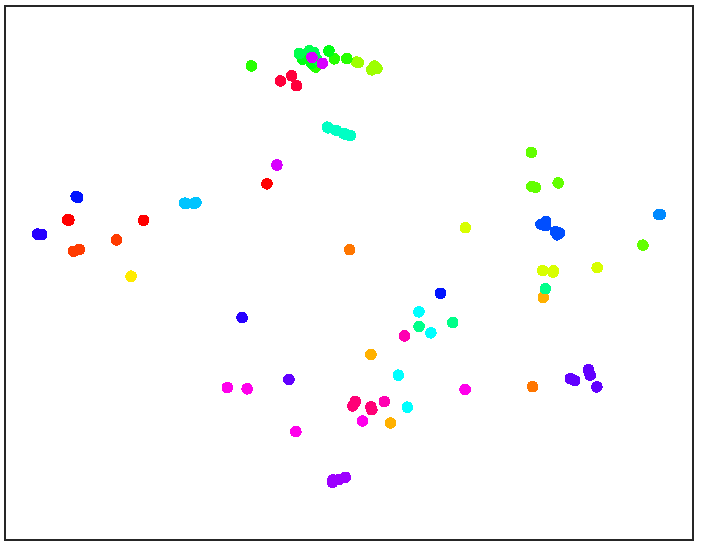
\includegraphics[width=1\textwidth]{./figures/C4Fig/tsne.eps}
		\end{minipage}%
	}%
	\subfigure[使用 STURE]{
		\begin{minipage}[t]{0.48\linewidth}
			\centering
			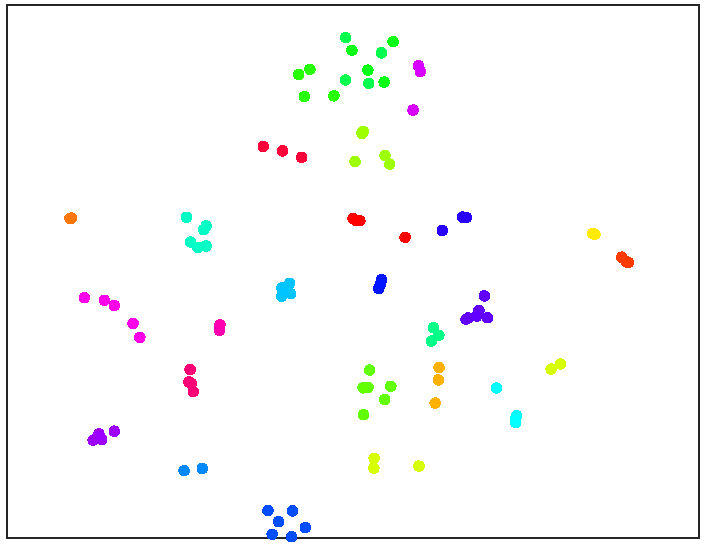
\includegraphics[width=1\textwidth]{./figures/C4Fig/tsne_best.eps}
		\end{minipage}%
	}%
	%\n is important,(or \quad) 
	
	\subfigure[未使用 STURE 的跟踪结果]{
		\begin{minipage}[t]{0.48\linewidth}
			\centering
			\includegraphics[width=1\textwidth]{./figures/C4Fig/tsne_tracking_result_without_STURE.pdf}
		\end{minipage}
	}%
	\subfigure[使用 STURE 的跟踪结果]{
		\begin{minipage}[t]{0.48\linewidth}
			\centering
			\includegraphics[width=1\textwidth]{./figures/C4Fig/tsne_tracking_result_with_STURE.pdf}
		\end{minipage}
	}%
	
	\centering
	\caption{互表征分布和跟踪结果的可视化
	}
	\label{fig:tsne}
\end{figure}


\subsubsection{非局部注意力模块}
非局部层用于提取目标序列中的时间表征。
为了证明添加的非局部层的有效性,删除它并使用经典的卷积神经网络结构来学习序列特征,
并且序列帧特征 $f_{Sn}$ 被替换为三维平均池化的序列特征。
在图~\ref{fig:sture_ablation} 中,如果删除非局部层,MOT16 和 MOT17 中的跟踪性能仍然大大超过了消去状态。
然而,去除 STURE 的跟踪性能低于删除非局部层。
与经典的三维池化操作相比,相信非局部层能够更好地提取时间特征,
并且它们还帮助检测学习网络更有效地学习时间特征。
此外,所提出的 STURE 在提高跟踪性能方面比非局部块重要得多。

在 MOT16 和 MOT17 基准测试中,从每种消去方法的性能相对于设计的完整方法(44.6$\%$)的跟踪性能可以看出,设计的每一个模块都对效果的提升做出了贡献。
如果将跟踪分数用于多目标跟踪,则 MOTA 急剧下降 8.1$\%$,这体现了 STURE 的优点。
禁用非局部层的性能下降证明非局部层比经典卷积架构更有效。



\vspace{0.5em}
\begin{figure*}[ht]
	\centering
	\includegraphics[width=0.8\textwidth]{./figures/C4Fig/ablation.pdf}
	\vspace{0.2em}
	\caption{基础模块的消去实验}
	\label{fig:sture_ablation}
\end{figure*}




\subsection{讨论}
所提出的 STURE 的鲁棒目标关联方法能很好地处理在线多目标跟踪中的轨迹关联,并在当前候选检测和历史轨迹之间执行目标关联。

\subsubsection{序列长度}
目标序列图像的数量是设计架构中跟踪性能的关键参数,
不同 $T$ 值的实验性能如图~\ref{fig:sture_T} 所示。
很容易发现,当 $T$ 设置为 $8$ 时,同时获得了最优的 MOTA 和 MOTP。

\vspace{0.5em}
\begin{figure*}[ht]
	\centering
	\includegraphics[width=0.8\textwidth]{./figures/C4Fig/T.pdf}
	\vspace{0.2em}
	\caption{在 MOT16 数据集上使用不同序列长度 $T$ 的效果}
	\label{fig:sture_T}
\end{figure*}


\subsubsection{跟踪的超参数}
此外,还进行了一些实验来表明各种阈值的影响,例如轨迹初始化、轨迹终止、外观相似性、跟踪分数和交并比。
跟踪参数在各种参数设置下进行测试。 
MOTA 随 $\tau_s$ 和 $\tau_a$ 的设置变化很大。
通过这种方式,$ \tau _s $ 和 $ \tau _a $ 基于训练的关联网络通过网格搜索进行选择。 
当 $ \tau _s=0.2 $ 和 $ \tau _a=0.8 $ 时,获得了最大化的 MOTA。 
因此,如前所示选择跟踪参数。


\vspace{0.5em}
\begin{figure*}[ht]
	\centering
	\includegraphics[width=1.0\textwidth]{./figures/C4Fig/tracking_result.pdf}
	\vspace{0.2em}
	\caption{在基准数据集上的跟踪结果示例}
	\label{fig:sture_tracking_result}
\end{figure*}

多目标跟踪的跟踪示例如图~\ref{fig:sture_tracking_result}~所示。
第一排是夜间拥挤的街道,高架相机视野的视频片段 MOT17-03、第二排是移动平台的街景的视频片段 MOT17-05 和从较低视角拍摄的拥挤行人环境视频片段 MOT17-09,当单目标跟踪过程在倒数第二列变为漂移状态时,所提出的算法可以很好地关联目标。
一般来说,当物体在相机中快速移动或受到其他物体的影响时,单目标跟踪器很容易漂移。
在这项工作中,提出了一个有效的关联方法被用来处理漂移。
此外,单目标跟踪器能够很好地解决遮挡问题。




\section{本章小结}
在这项研究中,提出了一种新的 STURE 方法,用于在线多目标跟踪任务中的鲁棒目标关联。
STURE 方法可以相互学习序列学习网络和检测学习网络中的时间表征。
通过互学习,检测学习网络可以学习时间特征并变得更加鲁棒,同时也将缓解当前检测结果与历史轨迹序列之间的特征不平衡问题。
并且通过当前检测结果与历史序列的关联来处理检测结果不完美的问题。
大量的实验证明了所设计方法的有效性,并且与目前存在的在线跟踪算法进行比较,表明所设计的算法可以在多目标跟踪基准上取得更好的性能。
 

